%! Author = Nilo
%! Date = 30/08/2019
% Preamble
\documentclass[a4paper,10pt,oneside]{book}
\usepackage{amssymb}
\usepackage{amsmath}
\usepackage{amsthm}
\usepackage{enumitem}
\usepackage{amsfonts}
\usepackage{xcolor}
\usepackage{tcolorbox}
\usepackage{float}
\usepackage{graphicx}
\usepackage{hyperref}

\colorlet{shadecolor}{gray!20}

\newcommand{\Date}{--/9-'19}
%
\newcommand{\questionBox}[1]{
\begin{tcolorbox}[width=\textwidth,
colback={shadecolor},
title={Question:},colbacktitle=white,coltitle=black]
    #1
\end{tcolorbox}
}
%
\newcommand{\answerBox}[1]{
\begin{tcolorbox}[width=\textwidth,
title={Answer:},colbacktitle=white,coltitle=black]
    #1
\end{tcolorbox}
}

\title{Prerequisites for Riemann Hypothesis}
\author{Nilo de Roock}
\date{\Date}

\begin{document}
    \maketitle
    %\newpage+
    \tableofcontents{}
    \newpage
    \thispagestyle{empty}


%    \chapter{Theorems}
%    \section{Complex Integration}


\begin{theorem}[Closed Contour Theorem (II.1.6)]
    \label{sec:ClosedContourT}
    If a continuous function
    $$ f : D \rightarrow \mathbb{C}, \qquad D \subset \mathbb{C} \quad \text{open},$$
    \textbf{has a primitive} then
    $$\oint_\alpha f(\zeta)d\zeta = 0$$
    for any piecewise smooth curve $\alpha$ in $\mathbb{C}$.
\end{theorem}


\begin{theorem}[Main Theorem Calculus (II.2.4)]
    \label{sec:MainTCalculus}
    For a continuous function
    $$ f : D \rightarrow \mathbb{C}, \qquad D \subset \mathbb{C} \quad \text{a domain},$$
    the following three statements are equivalent:
    \begin{enumerate}[label=\alph*)]
        \item $f$ has a primitive.
        \item The integral of $f$ along any closed curve in $D$ vanishes.
        \item The integral of $f$ along any curve in $D$ depends only on the beginning and end points of the curve.
    \end{enumerate}
\end{theorem}


\begin{theorem}[Cauchy Integral Theorem for Triangular Paths]
    \label{sec:CauchyITT}
    Let
    $$ f : D \rightarrow \mathbb{C}, \qquad D \subset \mathbb{C} \quad \text{open}$$
    be an analytic function (i.e. complex differentiable at any point $z \in D$). Let $z_1, z_2, z_3$ be three points
    in $D$ such that the triangle they span is also contained in D; then
    $$\int_{<z_1,z_2,z_3>} f(\zeta)d\zeta = 0.$$
\end{theorem}


\begin{theorem}[Cauchy Integral Theorem for Rectangular Paths]
    \label{sec:CauchyITR}
    Let \\
    TBD
\end{theorem}


\begin{theorem}[Cauchy Integral Formula]
    \label{sec:CauchyIF}
    Let \\
    TBD
\end{theorem}


\begin{theorem}[Generalized Cauchy Integral Formula]
    \label{sec:GCauchyIF}
    Let \\
    TBD
\end{theorem}


\begin{theorem}[Morera's Theorem]
    \label{sec:MoreraT}
    Let \\
    TBD
\end{theorem}


\begin{theorem}[Liouville's Theorem]
    \label{sec:LiouvilleT}
    Let \\
    TBD
\end{theorem}


\begin{theorem}[Fundamental Theorem of Algebra]
    \label{sec:FTAlgebra}
    Let \\
    TBD
\end{theorem}
%
%    \chapter{Strategies}
%
%    \chapter{Exercises}
%    \section{Complex Integration}
%
%    \subsection{Complex Line Integrals}
%    \section{FrBu II.1.1}
%    \section{FrBu II.1.2}

\questionBox{
    Let $\alpha : [0, \pi] \rightarrow \mathbb{C} $ be defined by
    $$\alpha(t) = e^{it}$$
    and $\beta : [0, 2] \rightarrow \mathbb{C} $ by

    \[
        \beta(t)=\left\{
        \begin{array}{lll}
            1 + t(-i-1) & \text{for } t \in [0,1]\\
            1 - t +i(t-2) & \text{for } t \in [1,2].
        \end{array}
        \right.
    \]

    Sketch $\alpha$, and $\beta$, and calculate

    $$ \int_{\alpha} \frac{1}{z} dz \text{ and } \int_{\beta} \frac{1}{z} dz.$$
}

\answerBox{
Sketch of $\alpha$, and $\beta$:

\begin{figure}[H]
    \centering
    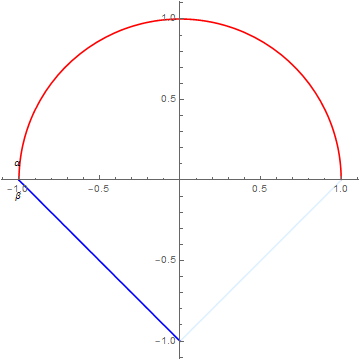
\includegraphics[width=0.5\textwidth]{pics/frbu212.png}
%   \caption{}
\end{figure}

Calculation of the integral along $\alpha$:
\begin{alignat*}{2}
    \int_{\alpha} \frac{1}{z} dz &= \int_{0}^{\pi} \frac{1}{e^{it}}i e^{it} dt &\qquad\hyperref[sec:ContourIntegral]{(1)} \\
    & = \int_{0}^{\pi} i dt & \\
    & = \left[ i t \right]_0^\pi & \\
    & = \pi i &
\end{alignat*}

Calculation of the integral along $\beta$:
\begin{equation*}
    \begin{split}
        \int_{\beta} \frac{1}{z} dz &= \int_0^1 \frac{-i-1}{1+t (-i-1)} \, dt+\int_1^2 \frac{-1+i}{1-2 i+t (-1+i)} \, dt \\
        & = \left[ \log (-1+(1+i) t) \right]_0^1 + \left[ \log ((-2-i)+(1+i) t) \right]_1^2 \\
        & = -\pi i
    \end{split}
\end{equation*}
}
%    \subsubsection{FrBu II.1.3}
%    \subsubsection{FrBu II.1.4}

\questionBox{
Sketch the following curve $\gamma$ ("figure eight")

\[
    \alpha(t)=\left\{
    \begin{array}{lll}
        1 - e^{i t} & \text{for } t \in [0,2 \pi]\\
        -1 + e^{-i t} & \text{for } t \in [2 \pi, 4 \pi].
    \end{array}
    \right.
\]

}

\answerBox{
Sketch of $\alpha$:

\begin{figure}[H]
    \centering
    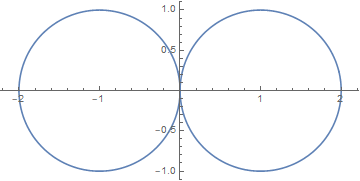
\includegraphics[width=0.5\textwidth]{pics/frbu214.png}
    %   \caption{}
\end{figure}
}
%    \section{FrBu II.1.5}

\questionBox{
Compute
$$\int_\alpha z^2 e^{z^2} dz,$$
where
\begin{enumerate}[label=\alph*)]
    \item $\alpha$ is the line between the point $0$ and the point $1 + i$,
    \item $\alpha$ is the piece of the parabola with equation $y = x^2$, which lies between the points $0$ and $1 + i$.
\end{enumerate}
}

\answerBox{
Calculation of the integral along $\alpha(t)=(1+i)t$:
\begin{alignat*}{2}
    \int_{\alpha} z e^{z^2} dz &= \int_{0}^{1} (1+i)e^{((1+i)t)^2} dt &\qquad\hyperref[sec:ContourIntegral]{(1)} \\
    & = \int_{0}^{1} 2it e^{2it^2} dt & \\
    & = \left[ \frac{1}{2}e^{2it^2} \right]_0^1 & \\
    & = \frac{1}{2}(e^{2i}-1) &
\end{alignat*}

Calculation of the integral along $\alpha(t)=t+it^2$:
\begin{alignat*}{2}
    \int_{\alpha} z e^{z^2} dz &= \int_{0}^{1} (t+it^2)e^{(t+it^2)^2} dt &\qquad\hyperref[sec:ContourIntegral]{(1)} \\
    & = \int_{0}^{1} (-2t^3+3it^2+t) e^{-t^4+2it^3+t^2} dt & \\
    & = \left[ \frac{1}{2}e^{-t^4+2it^3+t^2} \right]_0^1 & \\
    & = \frac{1}{2}(e^{2i}-1) &
\end{alignat*}

}
%    \subsubsection{FrBu II.1.6}

\questionBox{
Compute
$$\int_\alpha \sin(z) dz,$$
where $\alpha$ is the piece of the parabola with equation $y = x^2$, which lies between the points $0$ and $-1 + i$.
}

\answerBox{
Calculation of the integral along $\alpha(t)=-t+t^2i$:
\begin{alignat*}{2}
\int_{\alpha} \sin (z) dz &= \int_{0}^{1} \sin (-t+t^2i) (-1+2ti) dt &\qquad\hyperref[sec:ContourIntegral]{(1)} \\
& = \left[ -\cos (-t+t^2i) \right]_0^1 & \\
& = 1-\cosh (1+i) &
\end{alignat*}
}
%    \subsubsection{FrBu II.1.7}

\questionBox{
Let $[a,b]$ and $[c,d]$ ( $a < b$ and $c < d$ ) be compact intervals in $\mathbb{R}$. \\
\textit{Show:} there is an affine map
\begin{alignat*}{1}
    \varphi: [a,b] & \rightarrow [c,d], \\
    t & \mapsto \alpha t + \beta,
\end{alignat*}
with $\varphi(a)=c$ and $\varphi(b)=d$.
}

\answerBox{
If the map is
$$t \mapsto \frac{d-c}{b-a} t + \frac{cd - ad}{b-a}$$
then
\begin{alignat*}{1}
    \varphi(a): &= \frac{d-c}{b-a} a + \frac{cd - ad}{b-a}\\
    &= \frac{ad-ac+cb-ad}{b-a}\\
    &= \frac{cb-ac}{b-a}\\
    &=c
\end{alignat*}
and
\begin{alignat*}{1}
    \varphi(b): &= \frac{d-c}{b-a} b + \frac{cd - ad}{b-a}\\
    &= \frac{bd-bc+bc-ad}{b-a}\\
    &= \frac{bd-ad}{b-a}\\
    &=d.
\end{alignat*}
}
%    \subsubsection{FrBu II.1.8}

\questionBox{
Let $R>0$ be a positive number. We consider the curve
$$\beta = R e^{it}, 0 \leq t \leq \frac{\pi}{4}.$$
Show that:
$$|\int_\beta e^{iz^2} dz| \leq \frac{\pi(1-e^{-R^2})}{4R} < \frac{\pi}{4R}. $$
}

\answerBox{
[TBD] \\
Remark II.1.5 - Standard Estimate ???
}
%    \section{FrBu II.1.9}
%    \section{FrBu II.1.10}
%    \subsubsection{FrBu II.1.11}
%
%    \subsection{Cauchy Integral Theorem}
%    \section{FrBu II.2.1}
%    \subsubsection{FrBu II.2.2}
%    \subsubsection{FrBu II.2.3}
%    \subsubsection{FrBu II.2.4}
%    \subsubsection{FrBu II.2.5}

\questionBox{
Let $\alpha : [0, 1] \rightarrow \mathbb{C} $ with $\alpha(t) = e^{2 \pi t i}$
\begin{enumerate}[label=\alph*)]
    \item compute $\int_\alpha \frac{1}{|z|} dz$,
    \item compute $\int_\alpha \frac{1}{|z|^2} dz$,
    \item show that $|\int_\alpha \frac{1}{4+3z} dz| \le 2\pi$.
\end{enumerate}
}

\answerBox{
Calculation of the integral a).
\begin{alignat*}{2}
    \int_{\alpha} \frac{1}{|z|} dz &= \int_{0}^{1} \frac{1}{|e^{-2 i \pi  t}|}2 \pi i e^{2 i \pi  t} dt &\qquad\hyperref[sec:ContourIntegral]{(1)} \\
    & = \int_{0}^{1} 2 \pi  i e^{2 \pi i t} & \\
    & = \left[ e^{2 i \pi  t} \right]_0^1 & \\
    & = 0 &
\end{alignat*}

Calculation of the integral b).
\begin{alignat*}{2}
    \int_{\alpha} \frac{1}{|z|^2} dz &= \int_{0}^{1} \frac{1}{|e^{-2 i \pi  t}|^2}2 \pi i e^{2 i \pi  t} dt &\qquad\hyperref[sec:ContourIntegral]{(1)} \\
    & = \int_{0}^{1} 2 \pi  i e^{2 \pi i t} & \\
    & = \left[ e^{2 i \pi  t} \right]_0^1 & \\
    & = 0 &
\end{alignat*}

Calculation of the estimate of c).
\begin{alignat*}{2}
 & & \\
 & &
\end{alignat*}

[TBD] \\
Remark II.1.5 - Standard Estimate ???
}
%    \subsubsection{FrBu II.2.6}
%    \subsubsection{FrBu II.2.7}
%    \section{FrBu II.2.8}
%    \section{FrBu II.2.9}
%    \subsubsection{FrBu II.2.10}
%    \subsubsection{FrBu II.2.11}
%    \subsubsection{FrBu II.2.12}
%    \subsubsection{FrBu II.2.13}
%    \section{FrBu II.2.14}
%    \subsubsection{FrBu II.2.15}
%    \subsubsection{FrBu II.2.16}
%    \section{FrBu II.2.17}
%
%    \subsection{Cauchy Integral Formula}
%    \subsubsection{FrBu II.3.1}
%    \subsubsection{FrBu II.3.2}
%    \section{FrBu II.3.3}
%    \section{FrBu II.3.4}
%    \subsubsection{FrBu II.3.5}
%    \subsubsection{FrBu II.3.6}
%    \subsubsection{FrBu II.3.7}
%    \section{FrBu II.3.8}
%    \subsubsection{FrBu II.3.9}
%    \section{FrBu II.3.10}
%    \section{FrBu II.3.11}
%    \subsubsection{FrBu II.3.12}
%    \subsubsection{FrBu II.3.13}
%    \subsubsection{FrBu II.3.14}
%    \section{FrBu II.3.15}
%    \section{FrBu II.3.16}

    \chapter{Glossary}
    \section{Complex Integration}


\begin{definition}[Curve]
    \label{sec:Curve}
    Let\\
    TBD II.1.1
\end{definition}


\begin{definition}[Smooth Curve]
    \label{sec:SmoothCurve}
    Let\\
    TBD II.1.2
\end{definition}


\begin{definition}[Piecewise Smooth Curve]
    \label{sec:PiecewiseSmoothCurve}
    Let\\
    TBD II.1.3
\end{definition}


\begin{definition}[Contour Integral (II.1.4)]
    \label{sec:ContourIntegral}
    Let
    $$\alpha : [a, b] \rightarrow \mathbb{C}$$
    be a smooth curve and
    $$f: D \rightarrow \mathbb{C}, D \subset \mathbb{C},$$
    a continuous funtion, whose domain of definition contains the image of the curve $\alpha$,
    i.e. $D \supset \alpha([a,b]).$ Then one defines
    $$ \int_\alpha f:= \int_\alpha f(\zeta) d\zeta := \int_a^b f(\alpha(t))\alpha'(t)dt,$$
    and calls this complex number the line integral or \textbf{contour integral} of $f$ along $\alpha$.
    By the arc length of a smooth curve we mean
    $$l(\alpha):=\int_a^b |\alpha'(t)|dt.$$
\end{definition}


\begin{definition}[Properties Contour Integral (II.1.5)]
    \label{sec:PropContourIntegral}
    Let\\
    TBD
\end{definition}


\begin{definition}[Arcwise Connected Set (II.2.1)]
    \label{sec:ArcwiseConnected}
    Let\\
    TBD
\end{definition}


\begin{definition}[Domain (II.2.3)]
    \label{sec:Domain}
    Let\\
    TBD
\end{definition}


\begin{definition}[A Star-shaped Domain (II.2.6)]
    \label{sec:StarDomain}
    Let\\
    TBD
\end{definition}


\begin{definition}[Elementary Domain (II.2.8)]
    \label{sec:ElemDomain}
    Let\\
    TBD
\end{definition}

\end{document}